\section{RAID zero}

Data is inscribed onto a solitary logical disk and partitioned into multiple blocks dispersed across disks based on a striping algorithm. 
This method is preferred when prioritizing performance and capacity over reliability, necessitating a minimum of two drives. 
It offers cost-effectiveness since redundancy isn't utilized, meaning error-correcting codes aren't calculated or stored. 
It excels in write performance due to the absence of redundant data updates and parallelization.
However, a single disk failure can lead to irreversible data loss.

\subsection{Striping}
The core concept behind striping is to depict an array of disks as a unified large disk, thus maximizing parallelism by distributing data across all $N$ disks.
\begin{figure}[H]
    \centering
    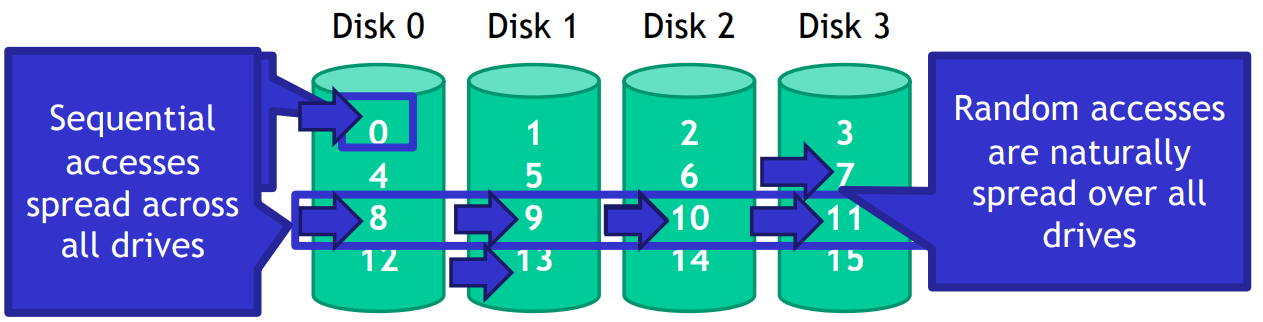
\includegraphics[width=1\linewidth]{images/strip.png}
    \caption{Data striping}
\end{figure}
Sequential accesses are evenly distributed across all drives, while random accesses occur naturally across all drives as well.
The access to a specific data blocks can be done by computing the number of disk, and the offset: 
\[\text{Disk}=\text{logical block number} \% \text{number of disks}\]
\[\text{Disk}=\dfrac{\text{logical block number}}{\text{number of disks}}\]

\paragraph*{Chunk sizing}
Chunk size influences array performance:
\begin{itemize}
    \item Smaller chunks lead to increased parallelism.
    \item Larger chunks result in reduced seek times.
\end{itemize}
Typical arrays utilize 64 kilobytes chunks.

\subsection{Summary}
The following is a summary of the features of RAID 0:
\begin{itemize}
\item The system has a capacity of $N$, meaning that it can hold all of the data on all drives.
\item The system has a reliability of $0$, meaning that if any drive fails, data will be permanently lost. 
    The Mean Time to Data Loss is equal to the Mean Time to Failure.
\item The system supports sequential read and write operations of $N\times S$, which means that data can be read and written in parallel across all drives.
\item The system also supports random read and write operations of $N\times R$, which means that data can be read and written in a random pattern across all drives.
\end{itemize}